%----------------------------------------------------------------------------------------
%	PACKAGES AND OTHER DOCUMENT CONFIGURATIONS
%----------------------------------------------------------------------------------------

\documentclass{article}

\usepackage{fancyhdr} % Required for custom headers
\usepackage{lastpage} % Required to determine the last page for the footer
\usepackage{extramarks} % Required for headers and footers
\usepackage[usenames,dvipsnames]{xcolor} % Required for custom colors
\usepackage{graphicx} % Required to insert images
\usepackage{listings} % Required for insertion of code
\usepackage{courier} % Required for the courier font
\usepackage{amsmath} % Used for matrices %
\usepackage{mathtools}
\usepackage{textcomp}
\usepackage{gensymb}
\usepackage{siunitx}
\usepackage{empheq}
\usepackage{ulem}
\usepackage{amssymb}
\usepackage[inline]{enumitem}

% Custom Commands %
\sisetup{output-exponent-marker=\ensuremath{\mathrm{E}}}
\definecolor{ao}{rgb}{0.0, 0.5, 0.0}

% Margins
\topmargin=-0.45in
\evensidemargin=0in
\oddsidemargin=0in
\textwidth=6.5in
\textheight=9.0in
\headsep=0.25in

\linespread{1.1} % Line spacing

% Set up the header and footer
\pagestyle{fancy}
\lhead{\hmwkAuthorName} % Top left header
\chead{\hmwkClass\ (\hmwkClassInstructor\ \hmwkClassTime): \hmwkTitle} % Top center head
\rhead{\firstxmark} % Top right header
\lfoot{\lastxmark} % Bottom left footer
\cfoot{} % Bottom center footer
\rfoot{Page\ \thepage\ of\ \protect\pageref{LastPage}} % Bottom right footer
\renewcommand\headrulewidth{0.4pt} % Size of the header rule
\renewcommand\footrulewidth{0.4pt} % Size of the footer rule

\setlength\parindent{0pt} % Removes all indentation from paragraphs

%----------------------------------------------------------------------------------------
%	CODE INCLUSION CONFIGURATION
%----------------------------------------------------------------------------------------

\definecolor{MyDarkGreen}{rgb}{0.0,0.4,0.0} % This is the color used for comments
\lstloadlanguages{Matlab} % Load Perl syntax for listings, for a list of other languages supported see: ftp://ftp.tex.ac.uk/tex-archive/macros/latex/contrib/listings/listings.pdf
\lstset{language=Matlab, % Use Perl in this example
        frame=single, % Single frame around code
        breakatwhitespace=true,
        breaklines = true,
        basicstyle=\small\ttfamily, % Use small true type font
        keywordstyle=[1]\color{Blue}\bf, % Perl functions bold and blue
        keywordstyle=[2]\color{Purple}, % Perl function arguments purple
        keywordstyle=[3]\color{Blue}\underbar, % Custom functions underlined and blue
        identifierstyle=, % Nothing special about identifiers                                         
        commentstyle=\usefont{T1}{pcr}{m}{sl}\color{MyDarkGreen}\small, % Comments small dark green courier font
        stringstyle=\color{Purple}, % Strings are purple
        showstringspaces=false, % Don't put marks in string spaces
        tabsize=5, % 5 spaces per tab
        %
        % Put standard Perl functions not included in the default language here
        morekeywords={rand},
        %
        % Put Perl function parameters here
        morekeywords=[2]{on, off, interp},
        %
        % Put user defined functions here
        morekeywords=[3]{test},
       	%
        morecomment=[l][\color{Blue}]{...}, % Line continuation (...) like blue comment
        numbers=left, % Line numbers on left
        firstnumber=1, % Line numbers start with line 1
        numberstyle=\tiny\color{Blue}, % Line numbers are blue and small
        stepnumber=1 % Line numbers go in steps of 1
        }

% Creates a new command to include a script, the first parameter is the filename of the script (without .pl), the second parameter is the caption
\newcommand{\script}[2]{
\begin{itemize}
\item[]\lstinputlisting[caption=#2,label=#1]{#1.m}
\end{itemize}
}

%----------------------------------------------------------------------------------------
%	DOCUMENT STRUCTURE COMMANDS
%	Skip this unless you know what you're doing
%----------------------------------------------------------------------------------------

% Header and footer for when a page split occurs within a problem environment
\newcommand{\enterProblemHeader}[1]{
\nobreak\extramarks{#1}{#1 continued on next page\ldots}\nobreak
\nobreak\extramarks{#1 (continued)}{#1 continued on next page\ldots}\nobreak
}

% Header and footer for when a page split occurs between problem environments
\newcommand{\exitProblemHeader}[1]{
\nobreak\extramarks{#1 (continued)}{#1 continued on next page\ldots}\nobreak
\nobreak\extramarks{#1}{}\nobreak
}

\setcounter{secnumdepth}{0} % Removes default section numbers
\newcounter{homeworkProblemCounter} % Creates a counter to keep track of the number of problems

\newcommand{\homeworkProblemName}{}
\newenvironment{homeworkProblem}[1][Problem \arabic{homeworkProblemCounter}]{ % Makes a new environment called homeworkProblem which takes 1 argument (custom name) but the default is "Problem #"
\stepcounter{homeworkProblemCounter} % Increase counter for number of problems
\renewcommand{\homeworkProblemName}{#1} % Assign \homeworkProblemName the name of the problem
\section{\homeworkProblemName} % Make a section in the document with the custom problem count
\enterProblemHeader{\homeworkProblemName} % Header and footer within the environment
}{
\exitProblemHeader{\homeworkProblemName} % Header and footer after the environment
}

\newcommand{\problemAnswer}[1]{ % Defines the problem answer command with the content as the only argument
\noindent\framebox[\columnwidth][c]{\begin{minipage}{0.98\columnwidth}#1\end{minipage}} % Makes the box around the problem answer and puts the content inside
}

\newcommand{\homeworkSectionName}{}
\newenvironment{homeworkSection}[1]{ % New environment for sections within homework problems, takes 1 argument - the name of the section
\renewcommand{\homeworkSectionName}{#1} % Assign \homeworkSectionName to the name of the section from the environment argument
\subsection{\homeworkSectionName} % Make a subsection with the custom name of the subsection
\enterProblemHeader{\homeworkProblemName\ [\homeworkSectionName]} % Header and footer within the environment
}{
\enterProblemHeader{\homeworkProblemName} % Header and footer after the environment
}

%----------------------------------------------------------------------------------------
%	NAME AND CLASS SECTION
%----------------------------------------------------------------------------------------

\newcommand{\hmwkTitle}{Assignment\ \#2} % Assignment title
\newcommand{\hmwkDueDate}{Thursday,\ October\ 15,\ 2015} % Due date
\newcommand{\hmwkClass}{CMSC\ 733} % Course/class
\newcommand{\hmwkClassTime}{11:00am} % Class/lecture time
\newcommand{\hmwkClassInstructor}{Aloimonos, Yiannis} % Teacher/lecturer
\newcommand{\hmwkAuthorName}{Kanishka Ganguly} % Your name

%----------------------------------------------------------------------------------------
%	TITLE PAGE
%----------------------------------------------------------------------------------------

\title{
\vspace{2in}
\textmd{\textbf{\hmwkClass:\ \hmwkTitle}}\\
\normalsize\vspace{0.1in}\small{Due\ on\ \hmwkDueDate}\\
\vspace{0.1in}\large{\textit{\hmwkClassInstructor\ \hmwkClassTime}}
\vspace{3in}
}

\author{\textbf{\hmwkAuthorName}}
\date{10/15/2015} % Insert date here if you want it to appear below your name

%----------------------------------------------------------------------------------------

\begin{document}

\maketitle

%----------------------------------------------------------------------------------------
%	TABLE OF CONTENTS
%----------------------------------------------------------------------------------------

%\setcounter{tocdepth}{1} % Uncomment this line if you don't want subsections listed in the ToC

\newpage
\tableofcontents
\newpage

%----------------------------------------------------------------------------------------
%	PROBLEM 1
%----------------------------------------------------------------------------------------
\begin{homeworkProblem}
\begin{homeworkSection}{(a)} 
\problemAnswer{
\begin{center}
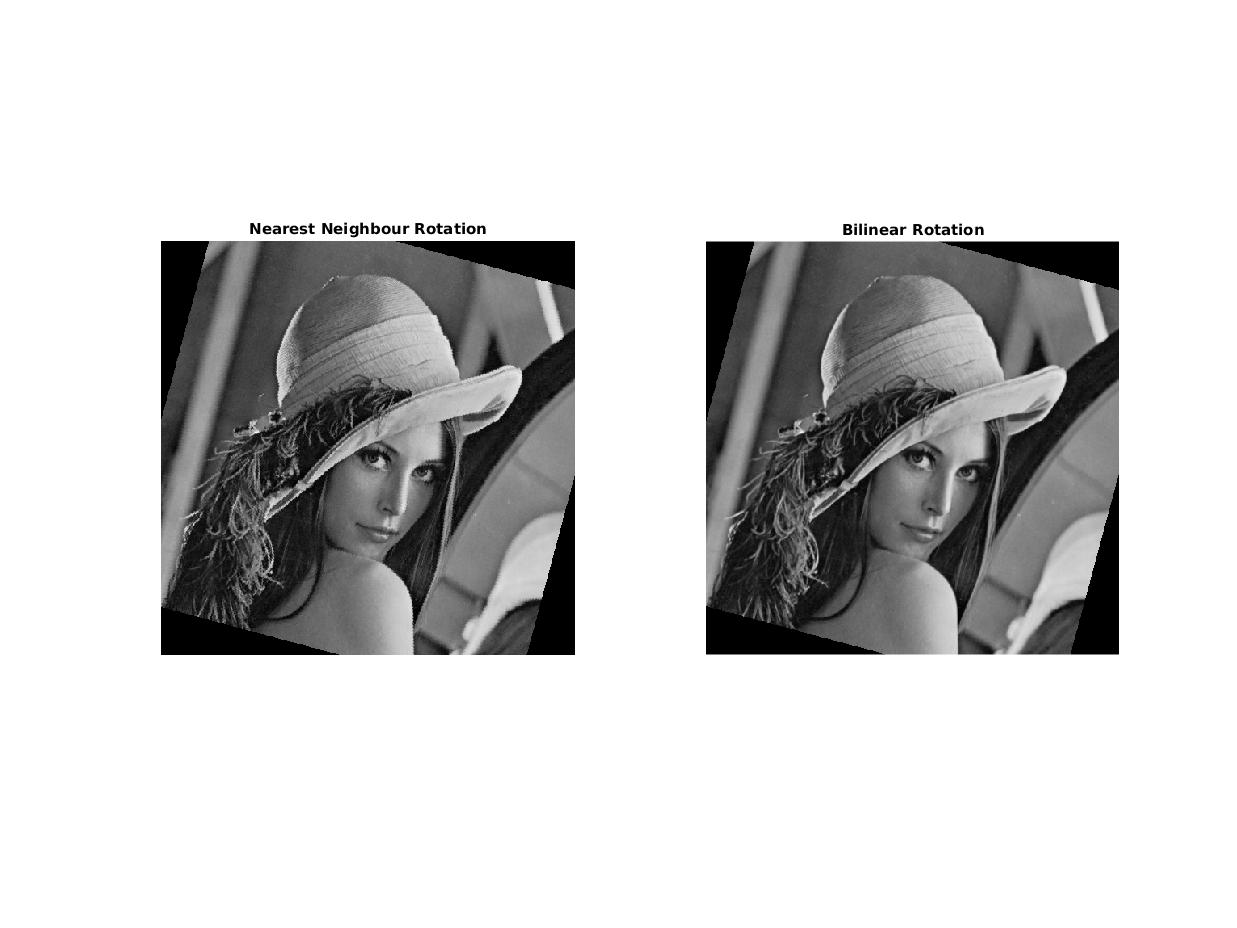
\includegraphics[width=0.75\columnwidth]{img/Q1_rotation.jpg}
\end{center}
}
\vspace{20pt}
Rotation of Image
\script{code/Q1_rotation}{Rotation}
\end{homeworkSection}

\begin{homeworkSection}{(b)} 
\problemAnswer{
\begin{center}
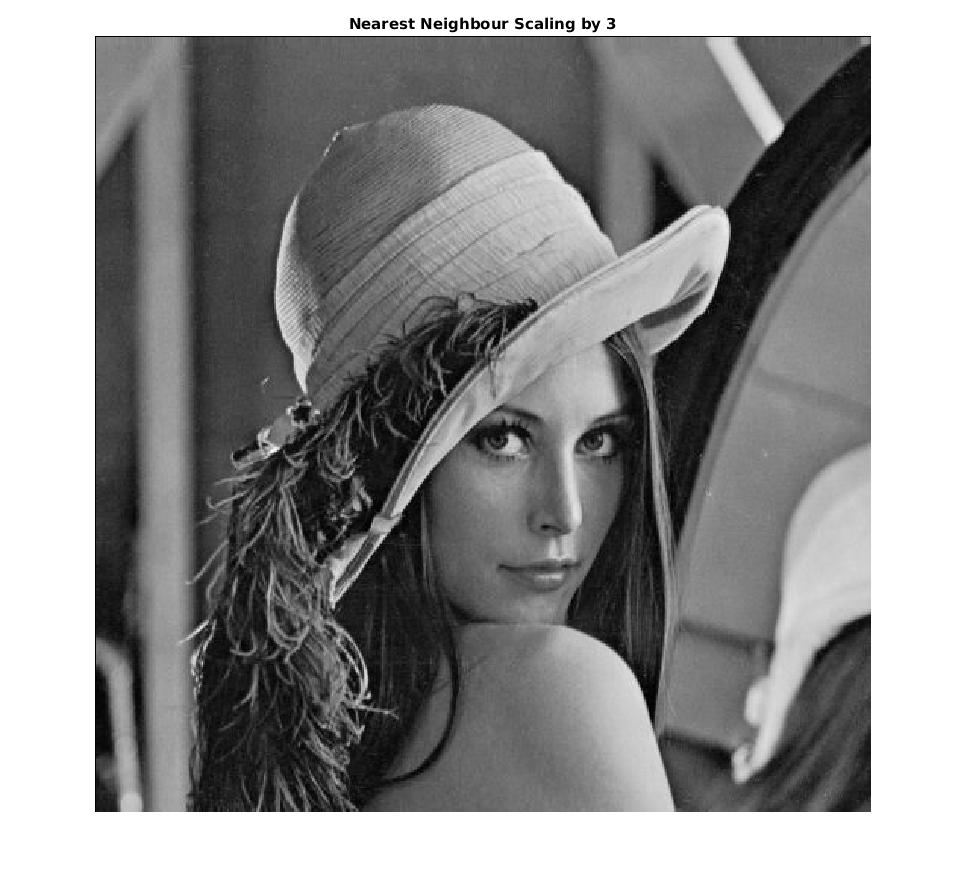
\includegraphics[width=0.75\columnwidth]{img/Q1_nnScale.jpg}
\end{center}
}
\vspace{20pt}
Nearest Neighbour Scaling of Image

\problemAnswer{
\begin{center}
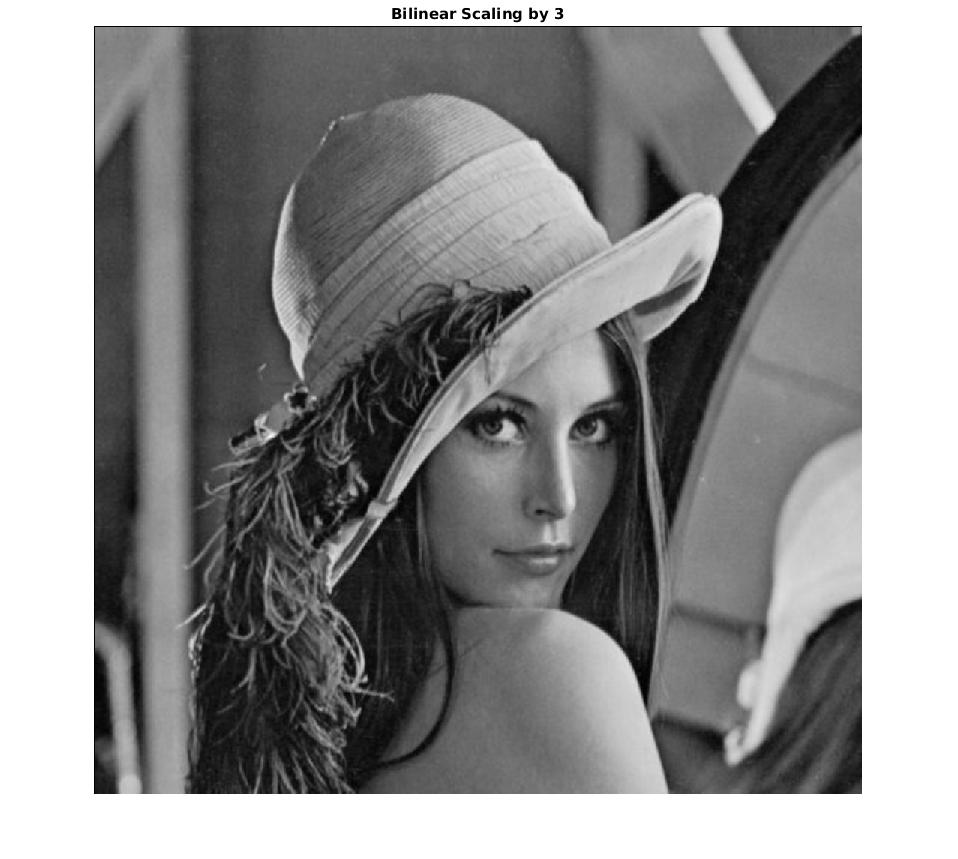
\includegraphics[width=0.75\columnwidth]{img/Q1_blScale.jpg}
\end{center}
}
\vspace{20pt}
Bilinear Scaling of Image
\script{code/Q1_scaling}{Scaling}
\end{homeworkSection}

\begin{homeworkSection}{(c)} 
\script{code/Q1_skewing}{Skewing}
\end{homeworkSection}

\begin{homeworkSection}{(d)} 
\script{code/Q1_affine}{Affine Transformation}

\problemAnswer{
\begin{center}
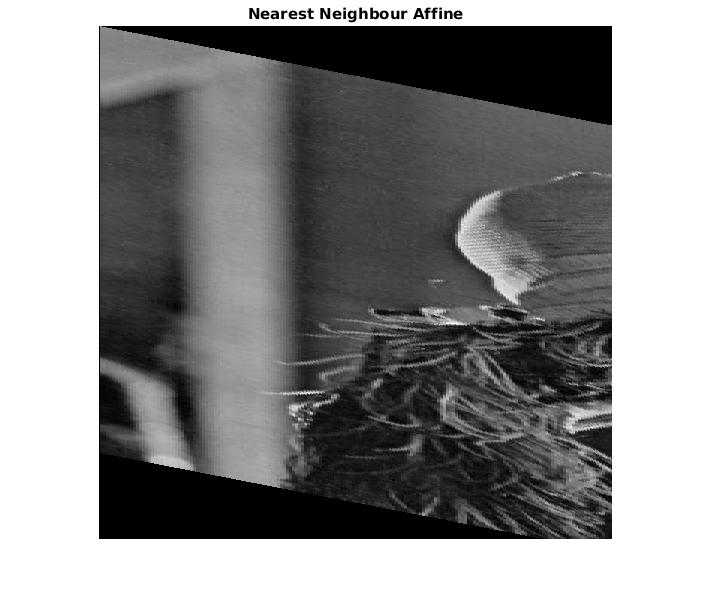
\includegraphics[width=0.75\columnwidth]{img/Q1_nnAffine.jpg}
\end{center}
}
\vspace{20pt}
Nearest Neighbour Affine Transform of Image

\problemAnswer{
\begin{center}
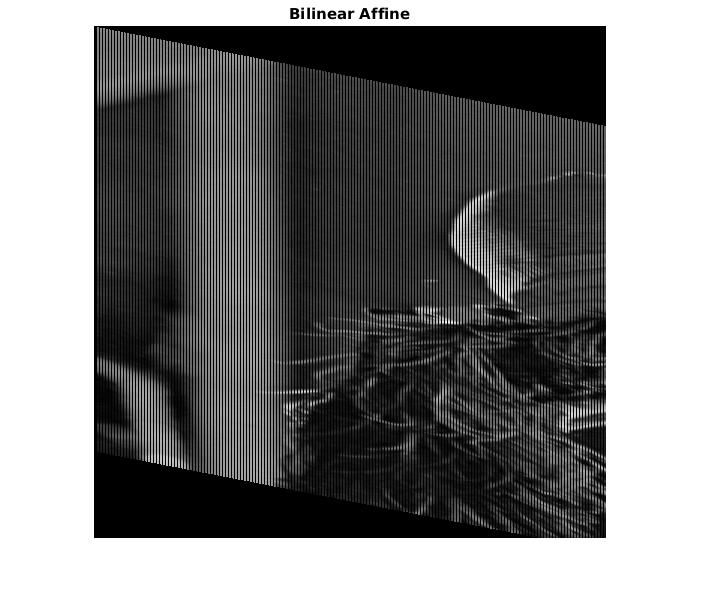
\includegraphics[width=0.75\columnwidth]{img/Q1_blAffine.jpg}
\end{center}
}
\vspace{20pt}
Bilinear Affine Transform of Image
\end{homeworkSection}
\end{homeworkProblem}
\clearpage
%----------------------------------------------------------------------------------------
%	PROBLEM 2
%----------------------------------------------------------------------------------------

\begin{homeworkProblem}
Given Image Patch as
\begin{align}
\begin{bmatrix}
9&10&9&4&3\\
5&7&8&9&3\\
4&5&6&8&5\\
3&4&5&6&8\\
2&3&4&5&6
\end{bmatrix}
\end{align}

\begin{homeworkSection}{(a)} 
\script{code/Q2_gaussian}{3x3 Gaussian Filter}
\script{code/Q2_box}{3x3 Box Filter}
\end{homeworkSection}

\begin{homeworkSection}{(b)} 
\script{code/Q2_sobel}{Sobel Edge Detector}

We get the following output:
\begin{verbatim}
edge_direction = 50.1944
edge_strength = 1.9526
\end{verbatim}
\end{homeworkSection}

\begin{homeworkSection}{(c)} 
\script{code/Q2_median}{Median Filter}

Median filtering has been shown to give best results for salt-and-pepper noise. Median filtering has the added advantage (over mean filters) of removing noise while preserving edges in an image (under certain conditions).\\
\begin{itemize}
\item Since the median is a more robust averaging technique than the mean, a single unrepresentative pixel in a neighbourhood will not affect the median value significantly. Thus, it is robust to the presence of outliers.
\item Also, since the median value must actually be the value of one of the pixels in the neighborhood, the median filter does not create new unrealistic pixel values when the filter straddles an edge. For this reason the median filter is much better at preserving sharp edges than the mean filter.
\end{itemize}
\end{homeworkSection}

\begin{homeworkSection}{(d)}
\uuline{Why the Gaussian is a good smoothing filter}
\begin{itemize}
\item A Gaussian filter is a better smoothing filter (as compared to the mean filter) because the Gaussian filter outputs a `weighted average' of each pixel's neighbourhood, where the average is weighted based on the distance each neighbouring pixel is away from the central pixel. So, pixels directly neighbouring the central pixel is weighted more than the ones farther away from the central pixel. This gives a much `gentler' smoothing and preserves edges better, as compared to a mean filter's uniformly weighted averaging technique.
\item Also, the Gaussian filter has a better \textit{frequency response} than the box (mean) filter. While both filters remove high spatial frequency components from an image, the Gaussian filter shows little to no oscillations in its frequency response as compared to the mean filter, which shows several oscillations.
\end{itemize}

\uuline{To perform Gaussian filtering fast}
\begin{itemize}
\item 
Gaussian filter has the property that it is separable, i.e. we can express the 2-D convolution as two 1-D convolutions. Thus, two 1-D convolutions can be performed in lesser time than one 2-D convolutions.
\item
If the filter is large, we can use the fact that a convolution in the spatial domain is equivalent to a multiplication in the frequency (Fourier) domain. This works well for multiple images, since we need to take the Fourier Transform of the Gaussian filter only once. Also, the set of Gaussian functions is closed under Fourier transforms, which means that the Fourier transform of a Gaussian is another Gaussian.
\end{itemize}
\end{homeworkSection}

\begin{homeworkSection}{(e)}
If the Gaussian kernel is larger than the width of the line, then after smoothing, the width of the line is reduced, i.e. the line becomes `thinner'. Also, at the edges of the line, we can see a `tapering' effect.
\end{homeworkSection}

\begin{homeworkSection}{(f)}
A box filter attenuates the noise because on taking the mean value of neighbouring pixels, the resulting output reduces the `variance' of the noise.\\
That is, the variance of noise in the mean is smaller than variance of the pixel noise.
\end{homeworkSection}

\end{homeworkProblem}
\clearpage

%----------------------------------------------------------------------------------------
%   PROBLEM 3
%----------------------------------------------------------------------------------------

\begin{homeworkProblem}
We have a 1-D image as follows:
\begin{align}
I(x) = cos(x/100)
\end{align}
When we apply gradient smoothing to $I(x)$, there is no effect on the intensity, which remains unchanged.\\
Thus, $I_{smooth} = cos(x/100)$.\\

On this smoothed image, when we calculate the derivatives, we use the mask $[-1 0 1]$. We see that the maximum absolute value (magnitude) of the derivative is obtained at $x = 100 [\pi/2 + n\pi]$. This is because the derivative of $cos(x)$ is $-sin(x)$, which is maximum at $\pi/2 + n\pi$. We can thus find the edges for the image at the zero-crossings of $cos(x/100)$.\\

Now, we see that the effect of increasing the $\sigma$ of the Gaussian filter doesn't affect the image since the intensities remain unchanged even after smoothing.\\
Also, an increase in the threshold value doesn't have any effect on the local maxima of the derivative since the maximum absolute value is still obtained at $x = 100 [\pi/2 + n\pi]$.
\end{homeworkProblem}
\clearpage

%----------------------------------------------------------------------------------------
%   PROBLEM 4
%----------------------------------------------------------------------------------------

\begin{homeworkProblem}
Let the given image $I$ be
\begin{align}
\begin{bmatrix}
1&2&3&4&5\\
3&4&5&6&7\\
5&6&\mathbf{7}&8&9\\
7&8&9&10&11\\
9&10&11&12&13
\end{bmatrix}
\end{align}

\begin{homeworkSection}{(a)}
For the gradient in the $x$-direction, we design a filter $K = \frac{1}{2}[-1 \quad 0 \quad 1]$.
Upon convolution with $f(x,y)$ we get $\frac{1}{2}[f(x+1,y) - f(x-1,y)]$ which is the gradient along the $x$-direction.\\
\begin{align}
\therefore gradient_x = \frac{8-6}{2} = 1
\end{align}

Similarly, to compute the gradient along the $y$-direction, we choose the filter $M = [-1 \quad 0 \quad 1]^T$.
\begin{align}
\therefore gradient_y = \frac{9-5}{2} = 2
\end{align}

The resultant gradient is given by:
\begin{align}
gradient_total = \sqrt{gradient_x^2 + gradient_y^2} = \sqrt{5}
\end{align}

To calculate the direction, we have $tan^{-1}(2) \degree$ with $x$-axis or $63.44 \degree$.
\end{homeworkSection}

\begin{homeworkSection}{(b)}
It is given that gradient at point $(3,7)$ is $(3,-2)$ and the intensity at that point is $17$.\\
We know that the gradient is defined as the change of intensity per unit distance, i.e. per pixel.\\
Thus we have
\begin{align}
I(3.1,7.3) = I(3,7) + G_x(0.1) + G_y(0.3)\\
\implies 17 + 0.3 -0.6 = 16.7
\end{align}
\end{homeworkSection}

\begin{homeworkSection}{(c)}
It is given that $I(x,y) = (x-5)^2 + (y-1)^2$\\
At $(x,y)$,
\begin{align}
gradient_x = \frac{1}{2}[ I(x+1, y) - I(x-1,y)] = -4\\
gradient_y = \frac{1}{2}[ I(x, y+1) - I(x,y-1)] = 2\\
\end{align}

\uuline{Thus we have gradient at $(3,2)$ as $(-4,2)$.}
\end{homeworkSection}
\end{homeworkProblem}
\clearpage

%----------------------------------------------------------------------------------------
%   PROBLEM 5
%----------------------------------------------------------------------------------------
\begin{homeworkProblem}
NOT ATTEMPTED
\end{homeworkProblem}
%----------------------------------------------------------------------------------------
%   PROBLEM 6
%----------------------------------------------------------------------------------------
\begin{homeworkProblem}
\script{code/Q6_histogram}{Main Routine}
\script{code/Q6_myColorHist}{Function \textit{myColorHist(I)}}
\script{code/Q6_histDist}{Function \textit{histDist(h1, h2)}}

For extra credit, I have developed a function that returns a percentage similarity between images that can be used to determine semantic similarity between scenes.
\script{code/Q6_similarity}{Function \textit{similarity(ssdR, ssdG, ssdB)}}
\problemAnswer{
\begin{center}
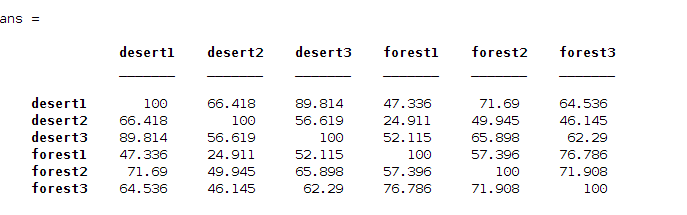
\includegraphics[width=0.75\columnwidth]{img/Q6.png}
\end{center}
}
\vspace{20pt}
Percentage Matrix for Semantic Similarity Determination Between Scenes

From the individual histograms of the Red, Green and Blue channels of two images, it may be determined whether two images are `similar' in which channel. This, combined with a precomputed set of `generic' values for each type of scene can be used to determine and differentiate between two scenes, such as a desert and a forest.\\
However, a more intelligent and adaptive algorithm than the one presented here is required, since it is evident from the values that in some cases, the presences of certain `unnecessary' features can dominate a histogram output.\\
For example, in a desert and a forest scene, if the `amount' of blue skies that are present dominate the `actual' desert and forest portions, then there would be a higher similarity being returned than what is expected.\\
Thus, along with color histograms, it might be necessary and useful to include other classification algorithms to detect `features' such as sand and trees in desert and forest scenes respectively.
\end{homeworkProblem}
\clearpage

%----------------------------------------------------------------------------------------
%   PROBLEM 7
%----------------------------------------------------------------------------------------
\begin{homeworkProblem}
NOT ATTEMPTED
\end{homeworkProblem}

%----------------------------------------------------------------------------------------
%   PROBLEM 8
%----------------------------------------------------------------------------------------
\begin{homeworkProblem}
\script{code/Q8_corner}{Corner Detection}
\problemAnswer{
\begin{center}
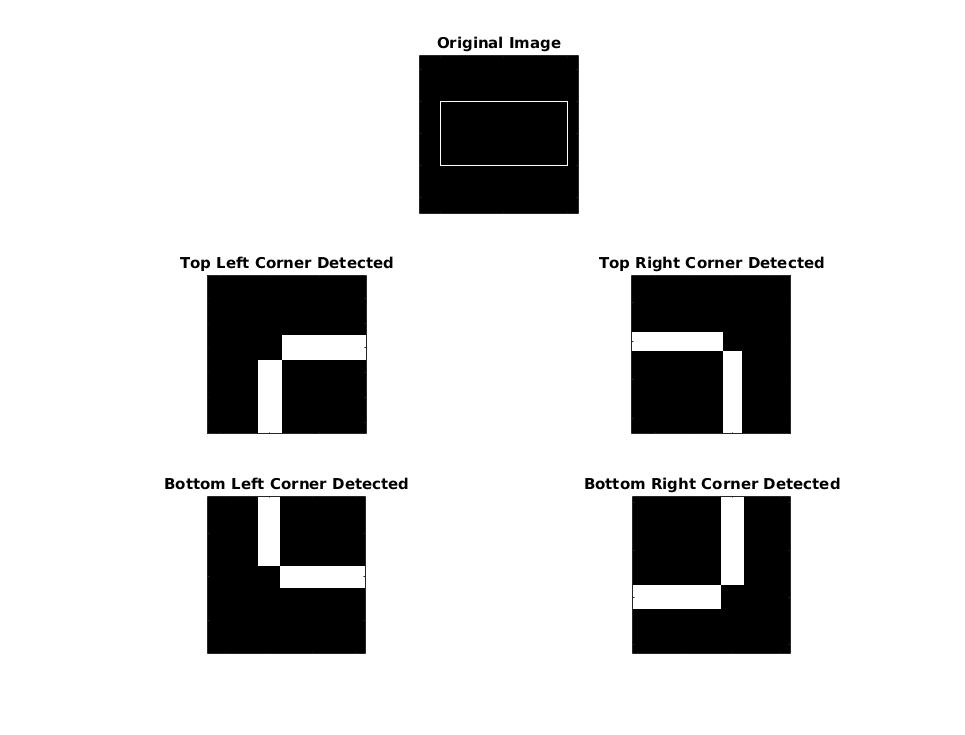
\includegraphics[width=0.75\columnwidth]{img/Q8.jpg}
\end{center}
}
\vspace{20pt}
All four corners detected and respective pixel removed for visualization

The algorithm proposed and demonstrated above uses the following masks:
\begin{align}
\text{Top Left Detector}=
\begin{bmatrix}
0 & 0 & 0 & 0 & 0\\
0 & 0 & 0 & 0 & 0\\
0 & 0 & 1 & 1 & 1\\
0 & 0 & 1 & 0 & 0\\
0 & 0 & 1 & 0 & 0\\
\end{bmatrix}\\
\text{Top Right Detector}=
\begin{bmatrix}
0 & 0 & 0 & 0 & 0\\
0 & 0 & 0 & 0 & 0\\
1 & 1 & 1 & 0 & 0\\
0 & 0 & 1 & 0 & 0\\
0 & 0 & 1 & 0 & 0\\
\end{bmatrix}\\
\text{Bottom Left Detector}=
\begin{bmatrix}
0 & 0 & 1 & 0 & 0\\
0 & 0 & 1 & 0 & 0\\
0 & 0 & 1 & 1 & 1\\
0 & 0 & 0 & 0 & 0\\
0 & 0 & 0 & 0 & 0\\
\end{bmatrix}\\
\text{Bottom Right Detector}=
\begin{bmatrix}
0 & 0 & 1 & 0 & 0\\
0 & 0 & 1 & 0 & 0\\
1 & 1 & 1 & 0 & 0\\
0 & 0 & 0 & 0 & 0\\
0 & 0 & 0 & 0 & 0\\
\end{bmatrix}\\
\end{align}

The algorithm works as follows:
\begin{enumerate}
\item Pad the image to make \textbf{ROWS} and \textbf{COLS} multiples of 5
\item Place respective mask over image, starting from top-left corner
    \begin{enumerate}
    \item Multiply mask element with image patch
    \item Calculate value for element $(3,3)$ and store as \textbf{BASELINE}
    \end{enumerate}
\item Traverse mask over image from \textbf{ROWS} to \textbf{COLS}
    \begin{enumerate}
    \item Multiply mask element with image patch
    \item Check if all non-zero elements of matrix are equal.
    \item IF EQUAL, compare value of non-zero element with \textbf{BASELINE}.
    \item IF EQUAL, corner is found. Break loop.
    \end{enumerate}
\item ELSE, REPEAT.
\end{enumerate}

This algorithm makes the assumption that the rectangle is made of lines which are 1 pixel thick and that the background is of uniform intensity.\\
It also assumes that the rectangle is anywhere within the bounds of the image and not touching any of the boundaries of the image.\\
This is a fairly robust algorithm since it can detect corners of multiple rectangles in the same image. Also, the entire algorithm can detect all four corners of a rectangle in one iteration, by placing all four masks in the same loop routine.\\
The main drawback of said algorithm is with boundary cases where any one edge of the rectangle is touching the edge of the image.
\end{homeworkProblem}
\clearpage
%----------------------------------------------------------------------------------------

%----------------------------------------------------------------------------------------
%   PROBLEM 9
%----------------------------------------------------------------------------------------
\begin{homeworkProblem}
\problemAnswer{
\begin{center}
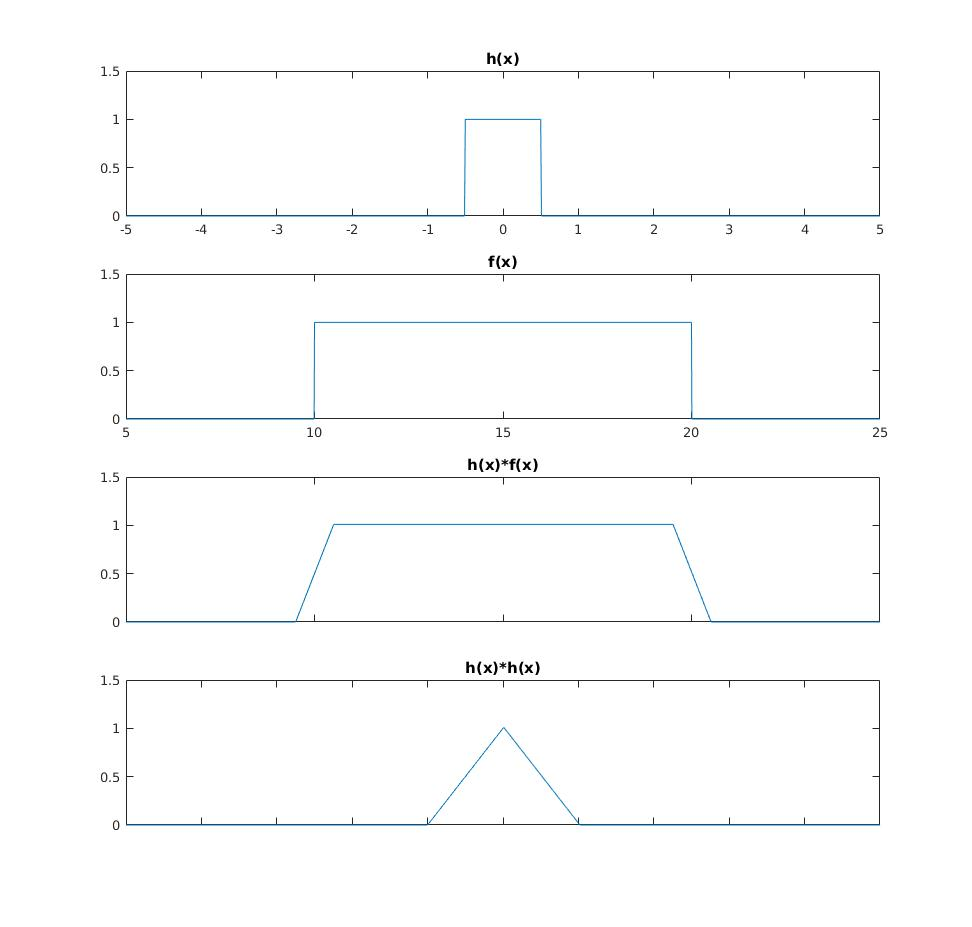
\includegraphics[width=0.75\columnwidth]{img/Q9.jpg}
\end{center}
}
\vspace{20pt}
Figures 
\begin{enumerate*}
\item $h(x)$
\item $f(x)$
\item $f(x) \ast h(x)$
\item $h(x) \ast h(x)$
\end{enumerate*}
\end{homeworkProblem}
\clearpage
%----------------------------------------------------------------------------------------

%----------------------------------------------------------------------------------------
%   PROBLEM 10
%----------------------------------------------------------------------------------------
\begin{homeworkProblem}
\begin{homeworkSection}{(a)}
Most images taken in a real-world situation (using normal cameras) have an inherent noise. Also, these images have several features that contain edges.\\
Taking derivates using finite differences is an operation that reduces the noise in the image. Also, using a smoothing filter such as a Gaussian causes these edges to blur, thus solving the problem of inhibiting the local edges that are unimportant to the analysis of the image, while retaining the more prominent, useful edges.
\end{homeworkSection}
\begin{homeworkSection}{(b)}
In the former implementation, i.e. convolving with Gaussian first and then taking the Laplacian, we first apply the Gaussian filter to the image using a discrete convolution and then apply the Laplacian operator. This requires two computations to the image, which decreases efficiency since the Gaussian filter needs to be applied to each image that we may have.\\
However, in the latter implementation, i.e. Laplacian of Gaussian, we can precompute the effect of the Laplacian on the Gaussian filter and then store and apply the resulting filter to the image. This reduces the computation time to just one major calculation, irrespective of the number of images we may have.
\end{homeworkSection}
\begin{homeworkSection}{(c)}
We can show that the Laplacian of the Gaussian is $G_1 \ast I - G_2 \ast I$ by taking
\begin{align}
LoG(x,y) = -\frac{1}{\pi \sigma^4} \bigg[ 1-\frac{x^2 + y^2}{2 \sigma^2} \bigg] e^{-\frac{x^2 + y^2}{2 \sigma^2}}
\end{align}
This equation can be approximated by using the difference of two Gaussian kernels with suitable values for $\sigma$. This ratio turns out to be $1:1.6$ for the best results.
\begin{align}
DoG = G_{\sigma_1} - G_{\sigma_2}\\
DoG = \frac{1}{2\pi} \bigg( \frac{1}{\sigma_1}e^{-\frac{x^2 + y^2}{2 \sigma_2^1}} - \frac{1}{\sigma_2}e^{-\frac{x^2 + y^2}{2 \sigma_2^2}} \bigg)
\end{align}
\end{homeworkSection}
\begin{homeworkSection}{(d)}
Difference of Gaussians $(DoG)$ is more efficient than Laplacian of Gaussian $(LoG)$ because one 2-D Gaussian operation is separable into two 1-D Gaussian operations, which is much more computationally efficient. Also, when transformed to the frequency domain, a Gaussian convolution operation becomes a multiplication operation. This also makes it more computationally efficient to calculate $(DoG)$ than $(LoG)$.
\end{homeworkSection}
\end{homeworkProblem}
\clearpage
%----------------------------------------------------------------------------------------

%----------------------------------------------------------------------------------------
%   PROBLEM 11
%----------------------------------------------------------------------------------------
\begin{homeworkProblem}
\script{code/Q11_sharpening}{Unsharp Sharpening}

\problemAnswer{
\begin{center}
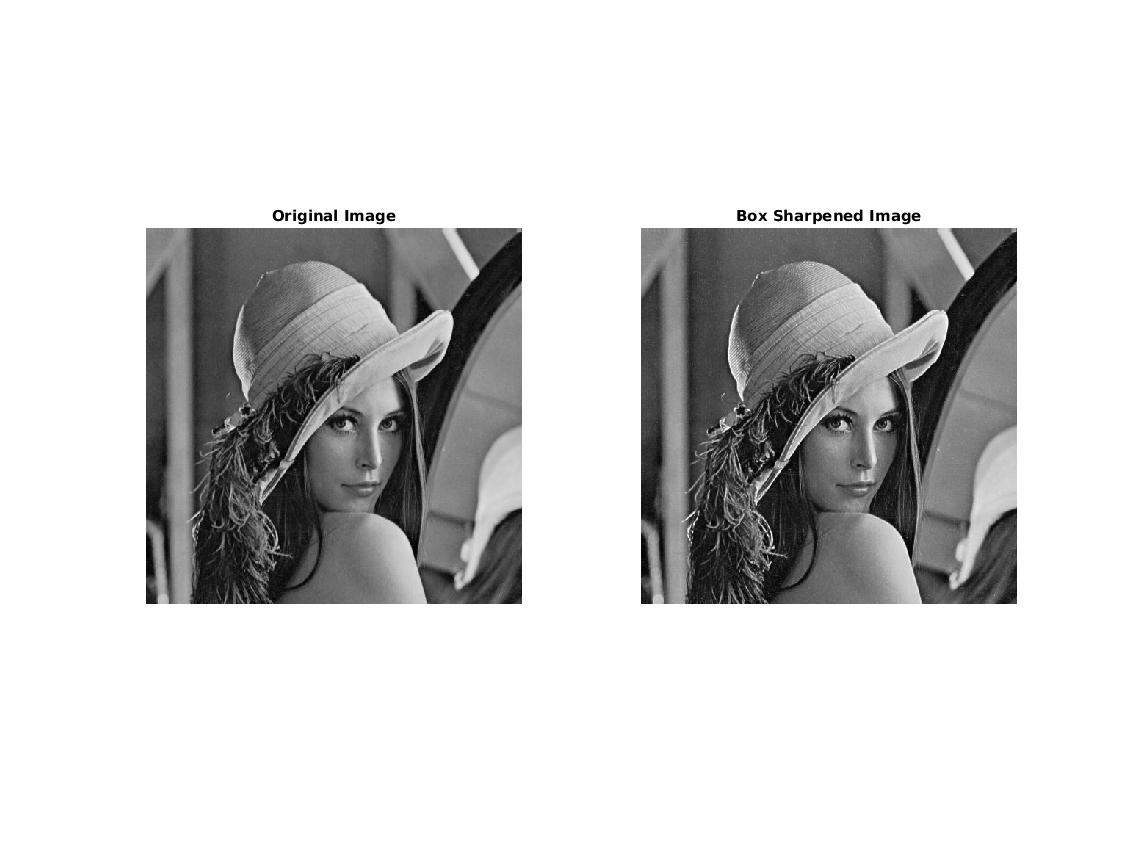
\includegraphics[width=0.75\columnwidth]{img/Q11_boxSharpen.jpg}
\end{center}
}
\vspace{20pt}
Unsharp Sharpening Using 3x3 Box Filter

By increasing kernel size, we get

\problemAnswer{
\begin{center}
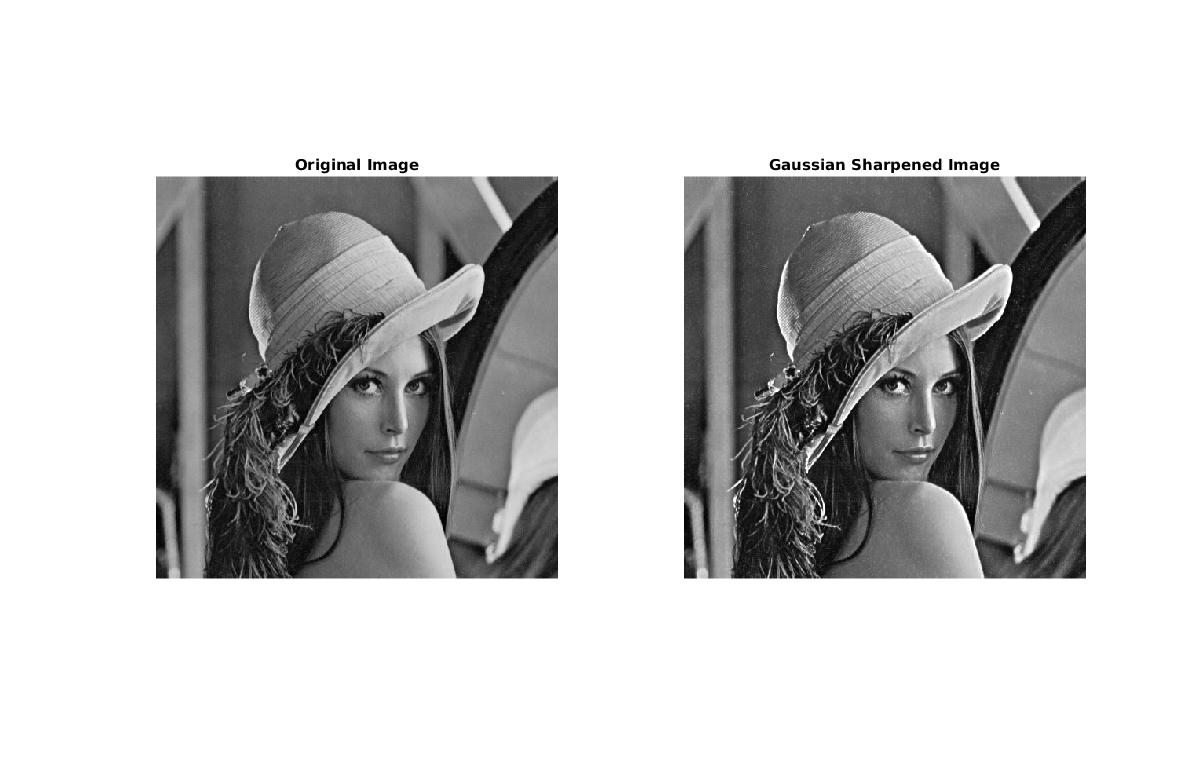
\includegraphics[width=0.75\columnwidth]{img/Q11_gaussSharpen4.jpg}
\end{center}
}
\vspace{20pt}
Unsharp Sharpening Using Gaussian Filter with $\sigma = 4$

\problemAnswer{
\begin{center}
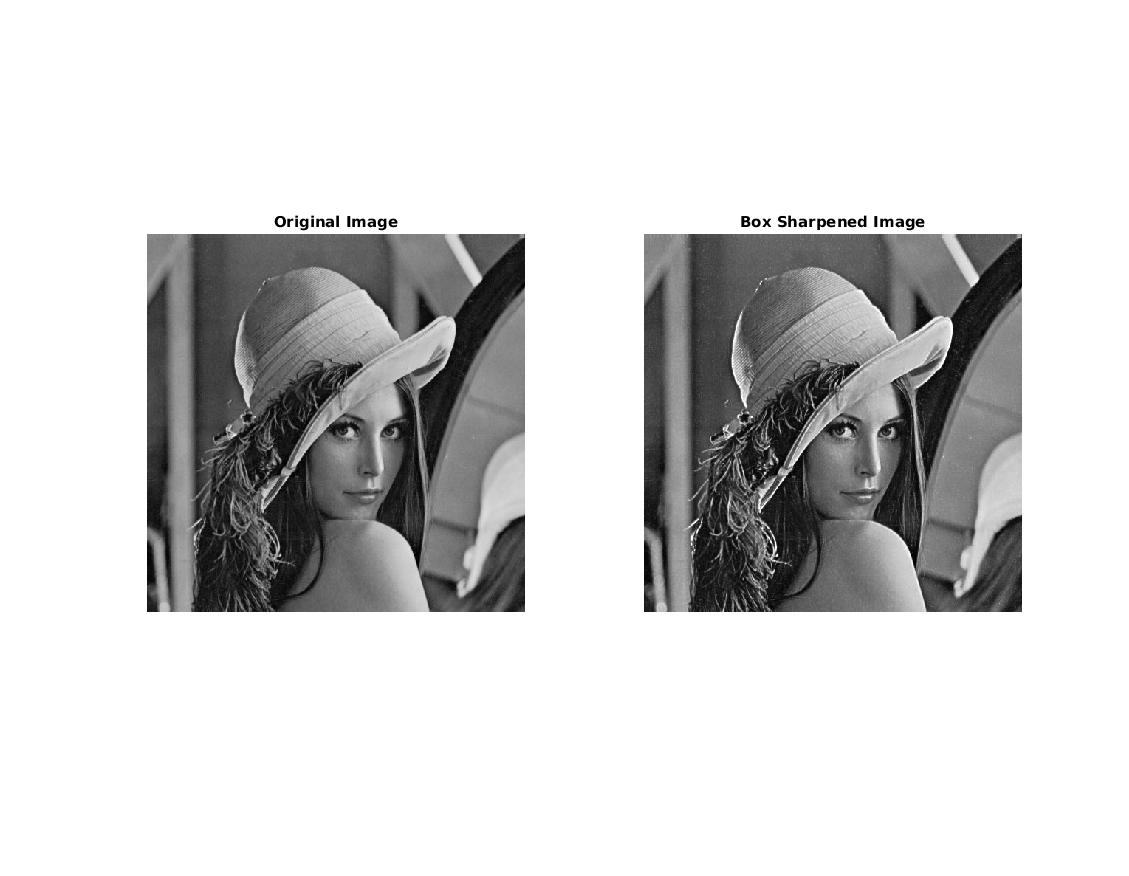
\includegraphics[width=0.75\columnwidth]{img/Q11_boxSharpen7x7.jpg}
\end{center}
}
\vspace{20pt}
Unsharp Sharpening Using 7x7 Box Filter
\end{homeworkProblem}
\clearpage
%----------------------------------------------------------------------------------------
\end{document}